
\documentclass{beamer}

\mode<presentation> {
\usetheme{Madrid}
}

\usepackage{graphicx}
\usepackage{booktabs} 

%----------------------------------------------------------------------------------------
%	TITLE PAGE
%----------------------------------------------------------------------------------------

\title[]{EE3025 - IDP} 

\author{Ch Pranay Prakash - EE18BTECH11009 }

\date{June 12, 2021} 

\begin{document}

\begin{frame}
\titlepage 
\end{frame}

%%%%%%%%%%%%%%%%%%%%%%%%%%%%%%%%%%%%%%%%%%%%%%%%%%%%%%%%%%%%%%%%%%%%%%%%%%%%%%%%
\begin{frame}
\frametitle{Problem}
\begin{enumerate}

    \item Let
    \begin{align}
        x(n) = \{{\underset{\uparrow}{1},2,3,4,2,1}\}
    \end{align}
    and 
    \begin{align}
        y(n) + \frac{1}{2}y(n-1) = x(n) + x(n-2) \\
        y(n) = 0 , n<0
        \label{eq:1.0.2}
    \end{align}
    Compute
    \begin{align}
        X(k) = \sum_{n=0}^{N-1}x(n)e^{-j2\pi kn/N},
        \quad k=0,1, \ldots, N-1
    \end{align}
    and H(k) using h(n).
\end{enumerate}
\end{frame}
%%=====================================================================================

\begin{frame}{Solution}
The Impulse response of an LTI system is the output of the system
when an Unit Impulse signal is given as the input to the system.\\
Now, giving Unit impulse signl as the input signal to the given system we get,
\begin{align}
    h(n) + \frac{1}{2}h(n-1) = \delta(n) + \delta(n-2)	
    \\
    \implies h(n) = \delta(n) + \delta(n-2) - \frac{1}{2}h(n-1) \label{eq:hn}
\end{align}
for N=6,
\begin{align}
     h(n) = \{{\underset{\uparrow}{1},-0.5,1.25,-0.625,0.3125,-0.15625}\}
\end{align}

\end{frame}
%%=====================================================================================
%%==============================================================================
%%%%%%%%%%%%%%%%%%%%%%%%%%% - N-point FFT Algorithm}
\begin{frame}
\frametitle{N-point FFT Algorithm}
The N-point DFT of a signal $x(n)$ is,
\begin{align}
    X(k) = \sum_{n=0}^{N-1}x(n)e^{-j2\pi kn/N},
    \quad k=0,1, \ldots, N-1 \label{eq:3dftx}
\end{align}

For the ease of calculation eq\eqref{eq:3dftx} can be broken down into two terms.
Even-indexed n term and odd-indexed n term.
\begin{align}
    X(k) &= \sum_{n=0(even-n)}^{N-1} x(n)W^{kn}_{N} + \sum_{n=0(odd-n)}^{N-1} x(n)W^{kn}_{N} \\
    &= \sum_{m=0}^{N/2 -1} x(2m)W^{2mk}_{N} + \sum_{m=0}^{N/2 -1} x(2m+1)W^{(2m+1)k}_{N} \\
    &= \sum_{m=0}^{N/2 -1} x(2m)W^{2mk}_{N} + W^{k}_{N} \sum_{m=0}^{N/2 -1} x(2m+1)W^{2mk}_{N} \label{eq:3.1.5}
\end{align}
\end{frame}

%========================================================================================
\begin{frame}
$\because$ complex exponential, $W_{N}^{nk}$ exhibits the following property,
\begin{align}
   (i) \quad W^{2}_{N} = W_{N/2}
\end{align}
\begin{align}
    [ \because (e^{-j2\pi kn/N})^2 = e^{-j2\pi kn/{(N/2)}}]
\end{align}
 using this property eq\eqref{eq:3.1.5} can be written as,
\begin{align}
    X(k) = \sum_{m=0}^{{N/2}-1} x(2m)W^{km}_{N/2} +W^{k}_{N} \sum_{m=0}^{{N/2}-1} x(2m+1)W^{km}_{N/2} \label{eq:3.1.8}
\end{align}
On comparing the above equation with the DFT equation \eqref{eq:3dftx}, we can observe that the first term is a N/2-point DFT of $x(2m)$ and second term is a N/2-point DFT of $x(2m+1)$. 
\end{frame}
%%%======================================================================================
\begin{frame}
    

Let,
\begin{align}
    X_{e}(k) &= \sum_{m=0}^{{N/2}-1} x(2m)W^{km}_{N/2} \\
    X_{o}(k) &= \sum_{m=0}^{{N/2}-1} x(2m+1)W^{km}_{N/2} \\
\end{align}
So, $X(k)$ can be written as,
\begin{align}
    X(k) = X_{e}(k) + W_{N}^k X_{o}(k) \label{eq:3.1.13}
\end{align}

From the above equation we can say that a N-point DFT is calculated from the sum of two N/2-point DFT.
\end{frame}
%%===================================================================================
\begin{frame}
Due to the periodicity of complex exponential function, $W_{N/2}^{nk}$ satisfies the following properties,
\begin{align}
  (ii) \quad W^{k+N/2}_{N/2} = W^{k}_{N/2}
\end{align}
\begin{align}
   [ \because e^{-j2\pi (k+N/2)/(N/2)} &= e^{-j2\pi k/(N/2)}.e^{-j2\pi  } \\
    &= e^{-j2\pi k/(N/2)}.1 \\
    &= e^{-j2\pi k/(N/2)} ]
\end{align}
\begin{align}
  (iii)\quad  W^{k+N/2}_{N} = -W^{k}_{N}\end{align}
\begin{align}
   [ \because e^{-j2\pi (k+N/2)/N} &= e^{-j2\pi k/N}.e^{-j\pi } \\
    &= e^{-j2\pi k/N}.(-1) \\
    &= -e^{-j2\pi k/N} ]
\end{align}
\end{frame}
%%====================================================================================

\begin{frame}
Replacing \{K\} with \{K+N/2\}, eq\eqref{eq:3.1.8} can be written as,
\begin{align}
    X(k+\frac{N}{2}) &= \sum_{m=0}^{{N/2}-1} x(2m)W^{m(k+\frac{N}{2})}_{N/2} +W^{k+\frac{N}{2}}_{N} \sum_{m=0}^{{N/2}-1} x(2m+1)W^{m(k+\frac{N}{2})}_{N/2}
\end{align}
Using properties (ii) and (iii), we have,
\begin{align}
    X(k+N/2) &= \sum_{m=0}^{{N/2}-1} x(2m)W^{mk}_{N/2} - W^{k}_{N} \sum_{m=0}^{{N/2}-1} x(2m+1)W^{mk}_{N/2} 
\end{align}
\begin{align}
    X(k+N/2) = X_{e}(k) - W_{N}^k X_{o}(k) \label{eq:3.1.25}
\end{align}
Now, from equations \eqref{eq:3.1.13} and \eqref{eq:3.1.25} i.e,
\begin{align}
    X(k) = X_{e}(k) + W_{N}^k X_{o}(k) \\
    X(k+N/2) = X_{e}(k) - W_{N}^k X_{o}(k) 
\end{align}
\end{frame}
%%====================================================================================
\begin{frame}
    

we have,
\begin{equation}
\begin{bmatrix}
X(0) \\
X(1) \\
X(2) \\
\vdots \\
X(${{$\frac{N}{2}$}-1}$)
\end{bmatrix}
= 
\begin{bmatrix}
X_{e}(0) \\
X_{e}(1) \\
X_{e}(2) \\
\vdots \\
X_{e}(${{$\frac{N}{2}$}-1}$)
\end{bmatrix}
+
\begin{bmatrix}
W^{0}_{N} & 0  &0 &. &. \\
0 & W^{1}_{N} & 0 & 0 &. \\
0 & 0 & W^{2}_{N} & 0 &. \\
\vdots & \vdots& & \ddots & \vdots\\
0 & 0 &. &. &W^{\frac{N}{2}-1}_{N}
\end{bmatrix}
\begin{bmatrix}
X_{o}(0) \\
X_{o}(1) \\
X_{o}(2) \\
\vdots \\
X_{o}(${{$\frac{N}{2}$}-1}$)
\end{bmatrix}
\end{equation}
\bigskip
\begin{equation}
\begin{bmatrix}
X(\frac{N}{2}) \\
X(\frac{N}{2}+1) \\
X(\frac{N}{2}+2) \\
\vdots \\
X(N)
\end{bmatrix}
= 
\begin{bmatrix}
X_{e}(0) \\
X_{e}(1) \\
X_{e}(2) \\
\vdots \\
X_{e}(${{$\frac{N}{2}$}-1}$)
\end{bmatrix}
-
\begin{bmatrix}
W^{0}_{N} & 0  &0 &. &. \\
0 & W^{1}_{N} & 0 & 0 &. \\
0 & 0 & W^{2}_{N} & 0 &. \\
\vdots & \vdots& & \ddots & \vdots\\
0 & 0 &. &. &W^{\frac{N}{2}-1}_{N}
\end{bmatrix}
\begin{bmatrix}
X_{o}(0) \\
X_{o}(1) \\
X_{o}(2) \\
\vdots \\
X_{o}(${{$\frac{N}{2}$}-1}$)
\end{bmatrix}
\end{equation}
\end{frame}

%%================================================================================

\begin{frame}{Conclusion (FFT Algorithm)}

In this way, by dividing the input signal into even and odd indices of n and using the properties of complex exponential we can calculate a N-point DFT by the sum of two N/2-point DFT's. Recursively we can further divide each N/2-point DFT into two N/4-point DFT's and so on. \\
\bigskip
The {\bf{FFT algorithm}} decreases the time complexity from $O(N^{2})$ to $O(NlogN)$, i.e, the DFT is computed faster. \\
\bigskip
\emph{Note: This algorithm is valid only when $N = 2^{m}$ for $m \in \mathbb{Z^{+}}$ is satisfied}

\end{frame}
%%%%%%%%%%%%%%%%%%%%%%%%%%%%%%%%%%%%%%%%%%%%%%%-- 8-point FFT ========================
\begin{frame}{8-point FFT algorithm}
Given input signal x(n),
\begin{align}
    x(n) = \{{\underset{\uparrow}{1},2,3,4,2,1} \}
\end{align}
For the given input signal N=6.\\
To satisfy $N = 2^{m}$, we have to zero-pad the input signal with the \\ closet $2^m$ value.\\
In this case it is 8($2^3$). \\
So we zero-pad the input signal with 2 zeros.
\begin{align}
    \implies x(n) = \{{\underset{\uparrow}{1},2,3,4,2,1,0,0}\}
\end{align}
Let $F_N$ be a N-point DFT matrix, then the DFT of $x(n)$ in the matrix form is given by,
\begin{align}
    X(k) = {F_{N}}.x(n)
\end{align}

\end{frame}
%%===================================================================================
\begin{frame}
For signal x(n) and $N=8$,\\
The 8-point DFT is given by,
\begin{align}
  X(k) = F_{8}.x(n)
\end{align}
Using the FFT algorithm we can write 8-point DFT in 4-point DFT's,
\begin{equation}
\begin{bmatrix}
X(0) \\ 
X(1) \\ 
X(2) \\ 
X(3)
\end{bmatrix}
=
\begin{bmatrix}
X_{e}(0) \\ 
X_{e}(1)\\ 
X_{e}(2)\\
X_{e}(3)\\
\end{bmatrix}
+
\begin{bmatrix}
W^{0}_{8} & 0 & 0 & 0\\
0 & W^{1}_{8} & 0 & 0\\
0 & 0 & W^{2}_{8} & 0\\
0 & 0 & 0 & W^{3}_{8}
\end{bmatrix}
\begin{bmatrix}
X_{o}(0) \\ 
X_{o}(1) \\ 
X_{o}(2) \\
X_{o}(3)
\end{bmatrix}
\end{equation}
\begin{equation}
\begin{bmatrix}
X(4) \\ 
X(5) \\ 
X(6) \\ 
X(7)
\end{bmatrix}
=
\begin{bmatrix}
X_{e}(0) \\ 
X_{e}(1)\\ 
X_{e}(2)\\
X_{e}(3)\\
\end{bmatrix}
-
\begin{bmatrix}
W^{0}_{8} & 0 & 0 & 0\\
0 & W^{1}_{8} & 0 & 0\\
0 & 0 & W^{2}_{8} & 0\\
0 & 0 & 0 & W^{3}_{8}
\end{bmatrix}
\begin{bmatrix}
X_{o}(0) \\ 
X_{o}(1) \\ 
X_{o}(2) \\
X_{o}(3)
\end{bmatrix}
\end{equation}
Here, 
\begin{align}
    X_{e} = F_{4}.[x(0),x(2),x(4),x(6)] \\
    X_{o} = F_{4}.[x(1),x(3),x(5),x(7)]
\end{align}
\end{frame}
%%=================================================================================
\begin{frame}
Now, from 4-point DFT's we get 2-point DFT's recursively,
\begin{equation}
\begin{bmatrix}
X_{e}(0) \\ 
X_{e}(1)\\ 
\end{bmatrix}
=
\begin{bmatrix}
X_{ee}(0) \\ 
X_{ee}(1)\\ 
\end{bmatrix}
+
\begin{bmatrix}
W^{0}_{4} & 0\\
0 & W^{1}_{4}
\end{bmatrix}
\begin{bmatrix}
X_{eo}(0) \\ 
X_{eo}(1) \\ 
\end{bmatrix}
\end{equation}


\begin{equation}
\begin{bmatrix}
X_{e}(2) \\ 
X_{e}(3)\\ 
\end{bmatrix}
=
\begin{bmatrix}
X_{ee}(0) \\ 
X_{ee}(1)\\ 
\end{bmatrix}
-
\begin{bmatrix}
W^{0}_{4} & 0\\
0 & W^{1}_{4}
\end{bmatrix}
\begin{bmatrix}
X_{eo}(0) \\ 
X_{eo}(1) \\ 
\end{bmatrix}
\end{equation}


\begin{equation}
\begin{bmatrix}
X_{o}(0) \\ 
X_{o}(1)\\ 
\end{bmatrix}
=
\begin{bmatrix}
X_{oe}(0) \\ 
X_{oe}(1)\\ 
\end{bmatrix}
+
\begin{bmatrix}
W^{0}_{4} & 0\\
0 & W^{1}_{4}
\end{bmatrix}
\begin{bmatrix}
X_{oo}(0) \\ 
X_{oo}(1) \\ 
\end{bmatrix}
\end{equation}


\begin{equation}
\begin{bmatrix}
X_{o}(2) \\ 
X_{o}(3)\\ 
\end{bmatrix}
=
\begin{bmatrix}
X_{oe}(0) \\ 
X_{oe}(1)\\ 
\end{bmatrix}
-
\begin{bmatrix}
W^{0}_{4} & 0\\
0 & W^{1}_{4}
\end{bmatrix}
\begin{bmatrix}
X_{oo}(0) \\ 
X_{oo}(1) \\ 
\end{bmatrix}
\end{equation}
\end{frame}
%%==================================================================================
\begin{frame}
    

Here,
\begin{align}
    X_{ee} &= [X_{e}(0),X_{e}(2)] \\
    &=F_{2}.[x(0),x(4)]
\end{align}
\begin{align}
    X_{eo} &= [X_{e}(1),X_{e}(3)]\\
    &=F_{2}.[x(2),x(6)]
\end{align}
\begin{align}
    X_{oe} &= [X_{o}(0),X_{o}(2)] \\
    &=F_{2}.[x(1),x(5)]
\end{align}
\begin{align}
    X_{oo} &= [X_{o}(1),X_{o}(3)]\\
    &=F_{2}.[x(3),x(7)]
\end{align}
\end{frame}
%%%===================================================================================
\begin{frame}
Now, 2-point DFT Matrix is given by, 
\begin{equation}
\because
F_{2} =
\begin{bmatrix}
1 & 1 \\
1&-1
\end{bmatrix}
\end{equation}
$\implies$ we get,
\begin{equation}
\begin{bmatrix}
X_{ee}(0) \\ 
X_{ee}(1)\\ 
\end{bmatrix}
= F_{2}
\begin{bmatrix}
x(0) \\ 
x(4) \\ 
\end{bmatrix}
=
\begin{bmatrix}
x(0)+x(4) \\ 
x(0)-x(4) \\ 
\end{bmatrix}
\end{equation}
\begin{equation}
\begin{bmatrix}
X_{eo}(0) \\ 
X_{eo}(1)\\ 
\end{bmatrix}
= F_{2}
\begin{bmatrix}
x(2) \\ 
x(6) \\ 
\end{bmatrix}
=
\begin{bmatrix}
x(2)+x(6) \\ 
x(2)-x(6) \\ 
\end{bmatrix}
\end{equation}
\begin{equation}
\begin{bmatrix}
X_{oe}(0) \\ 
X_{oe}(1)\\ 
\end{bmatrix}
= F_{2}
\begin{bmatrix}
x(1) \\ 
x(5) \\ 
\end{bmatrix}
=
\begin{bmatrix}
x(1)+x(5) \\ 
x(1)-x(5) \\ 
\end{bmatrix}
\end{equation}
\begin{equation}
\begin{bmatrix}
X_{oo}(0) \\ 
X_{oo}(1)\\ 
\end{bmatrix}
= F_{2}
\begin{bmatrix}
x(3) \\ 
x(7) \\ 
\end{bmatrix}
=
\begin{bmatrix}
x(3)+x(7) \\ 
x(3)-x(7) \\ 
\end{bmatrix}
\end{equation}
\end{frame}
%%=====================================================================================

%----------------------------------------------------------------------------------------
\begin{frame}{x(n)}
\begin{figure}[h!]
    \centering
    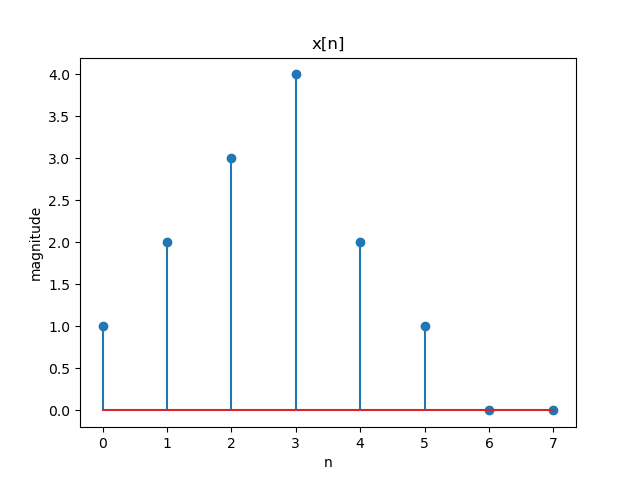
\includegraphics[height=6.8cm,width=9cm]{x_fft.png}
    \label{figs}
\end{figure}
\end{frame}


\begin{frame}{Amplitude of X(k)}
\begin{figure}[h!]
    \centering
    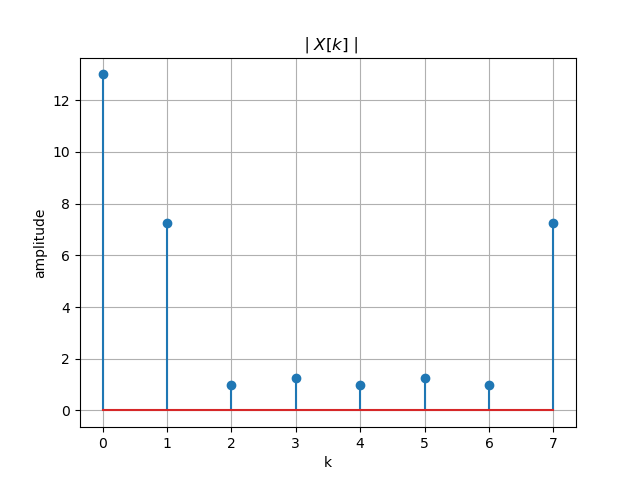
\includegraphics[height=6.8cm,width=9cm]{Xamp_fft.png}
    \label{figs}
\end{figure}
\end{frame}

\begin{frame}{Phase of X(k)}
\begin{figure}[h!]
    \centering
    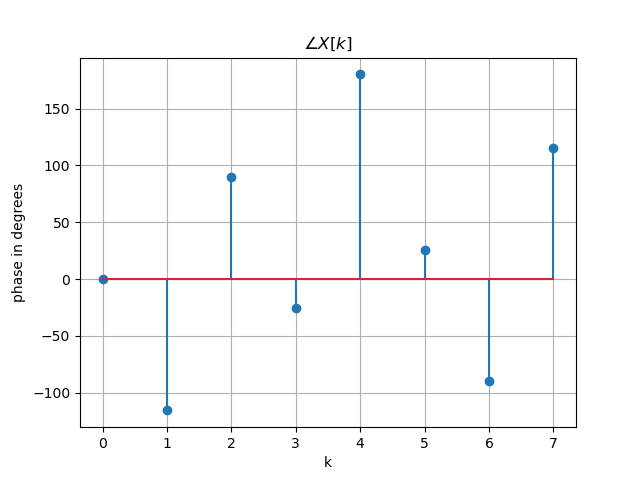
\includegraphics[height=6.8cm,width=9.5cm]{Xpha_fft.png}
    \label{figs}
\end{figure}
\end{frame}




\begin{frame}{h(n)}
\begin{figure}[h!]
    \centering
    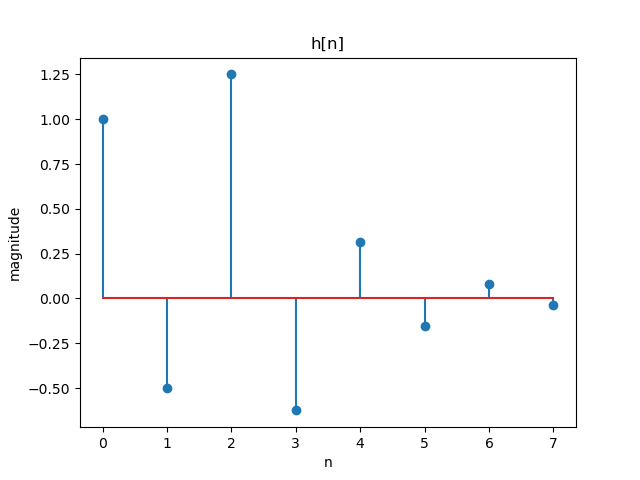
\includegraphics[height=6.8cm,width=9cm]{h_fft.png}
    \label{figs}
\end{figure}
\end{frame}





\begin{frame}{Amplitude of H(k)}
\begin{figure}[h!]
    \centering
    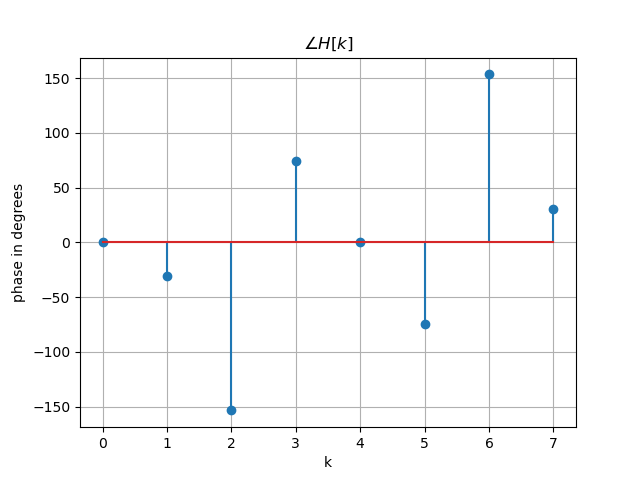
\includegraphics[height=6.8cm,width=9.5cm]{Hpha_fft.png}
    \label{figs}
\end{figure}
\end{frame}

\begin{frame}{Phase of H(k)}
\begin{figure}[h!]
    \centering
    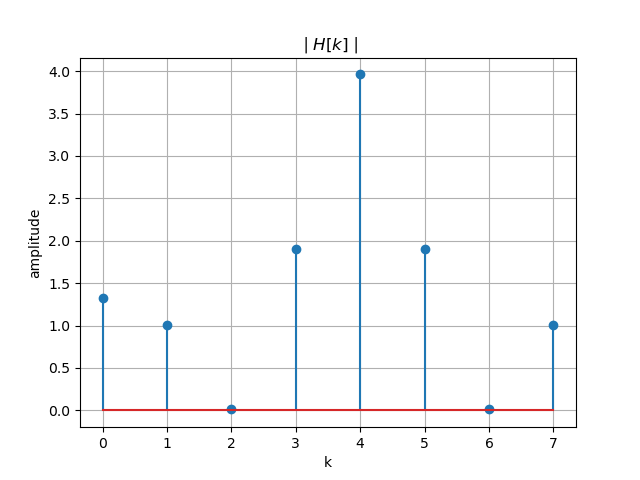
\includegraphics[height=6.8cm,width=9.25cm]{Hamp_fft.png}
    \label{figs}
\end{figure}
\end{frame}


\begin{frame}
\Huge{\centerline{The End}}
\end{frame}
\end{document}